\documentclass[final, 18pt]{beamer}
\usepackage[scale=1.24]{beamerposter}
\usepackage{beamerthemeconfposter}

\setbeamercolor{alertblock title}{fg=BrickRed,bg=white} % Colors of the alertblock titles

\newlength{\sepwid}
\newlength{\onecolwid}
\setlength{\paperwidth}{48in} % A0 width: 46.8in
\setlength{\paperheight}{36in} % A0 height: 33.1in
\setlength{\sepwid}{0.024\paperwidth} % Separation width (white space) between columns
\setlength{\onecolwid}{0.3\paperwidth} % Width of one column
\setlength{\topmargin}{0.25in} % Reduce the top margin size
%-----------------------------------------------------------

\usepackage{graphicx}
\usepackage{booktabs}

% --- title section ---
\title{Dynamic RNN State Updates for Irregular\\ Multivariate Time Series Classification}
\author{Tom Hartvigsen, Cansu Sen, Xiangnan Kong, Elke Rundensteiner}
\institute{Data Science, Worcester Polytechnic Institute}

%----------------------------------------------------------------------------------------

\begin{document}
\addtobeamertemplate{alertblock end}{}{\vspace*{24ex}} % White space under alertblocks
\addtobeamertemplate{alertblock example end}{}{\vspace*{2ex}} % White space under example alertblocks
\addtobeamertemplate{alertblock alerted end}{}{\vspace*{2ex}} % White space under highlighted (alert) alertblocks

\setlength{\belowcaptionskip}{2ex} % White space under figures
\setlength\belowdisplayshortskip{2ex} % White space under equations
%\begin{darkframes} % Uncomment for dark theme, don't forget to \end{darkframes}
\begin{frame} % The whole poster is enclosed in one beamer frame

\vspace{-3.5cm} % Space between blocks and header

\begin{columns}[t] % The whole poster consists of three major columns, the second of which is split into two columns twice - the [t] option aligns each column's content to the top

\begin{column}{\sepwid}\end{column} % Empty spacer column

\begin{column}{\onecolwid} % The first column

\begin{alertblock}{Irregular Multivariate Time Series}
Variables have different sampling rates. Empty spaces between observations can be informative. Prior to classification, timestamps must be aligned.
\\
Three common challenges with such data:
\begin{itemize}
    \item Irregular observation rates require time-alignment.
    \item Missing values may or may not be informative.
    \item High sampling-rate lead to long sequences. As dependencies grow over time, it becomes more challenging to remember only useful information.
\end{itemize}
\end{alertblock}

% --- problem definition ---
\begin{alertblock}{\centering Problem Setting}
\begin{figure}
    \centering
    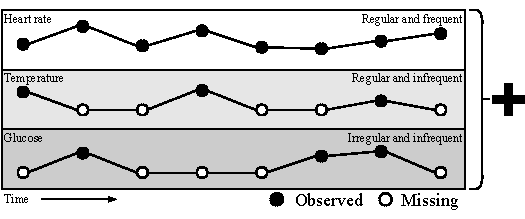
\includegraphics[width=.9\onecolwid]{./img/problem_definition.pdf}
\end{figure}
\end{alertblock}


% --- traditional approaches ---
\begin{alertblock}{\centering Traditional approaches}
\begin{itemize}
    \item Up-sampling slow variables vs. down-sampling fast variables.
    \item Combinations of different information sources (time delta, masking vector) are fed to RNNs.
    \item Some approaches also try to find meaningful values to impute.
\end{itemize}

\begin{figure}
    \centering
    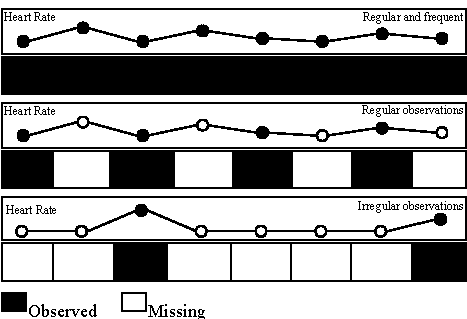
\includegraphics[width=.8\onecolwid]{./img/additional_information.pdf}
\end{figure}
\end{alertblock}

\end{column} % End column one

% --- spacer ---
\begin{column}{\sepwid}\end{column}

% --- new column ---
\begin{column}{\onecolwid}

\begin{alertblock}{\centering Missingness-Informed State-Skipping RNN}
\textit{Intuition}: Update the cell memory only when useful information is observed.

\begin{figure}
    \centering
    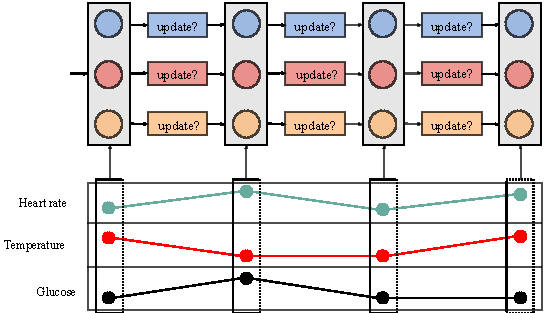
\includegraphics[width=.9\onecolwid]{img/MISS_mechanics.pdf}
    \caption{Mechanics of partial state-updates.}
\end{figure}

Representation generation in MISS-RNN:
\begin{align*}
    \gamma_t &= -\exp\{-max(0, W_\gamma\cdot\delta_t + b_\gamma)\} \\
    \hat{x_t} &= m_t x_t + (1-m_t)(\gamma_{x_t} x_{t^\prime} + (1-\gamma_{x_t})\tilde{x})\\
    \hat{S}_{t-1} &= \gamma_{S_t}*S_{t-1}\\
    \tilde{S_t} &= \text{GRU}([\hat{x_t}, m_t], \hat{S}_{t-1})\\
    u_t &= \text{binarize}(\sigma(W_s\cdot \tilde{S_t} + b_s)),\ \text{s.t.}\ u_t \in \mathbb{R}^h\\
    S_t &=  u_t \odot \tilde{S_t} + (1-u_t) \odot S_{t-1}
\end{align*}

\vspace{0.5cm}
\begin{figure}
    \centering
    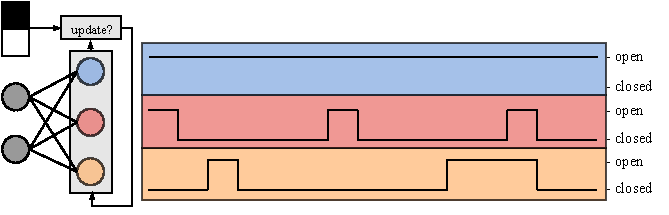
\includegraphics[width=.9\onecolwid]{img/MISS_effect.pdf}
    \caption{Resulting dynamics in hidden state updates patterns.}
\end{figure}

\begin{figure}
    \centering
    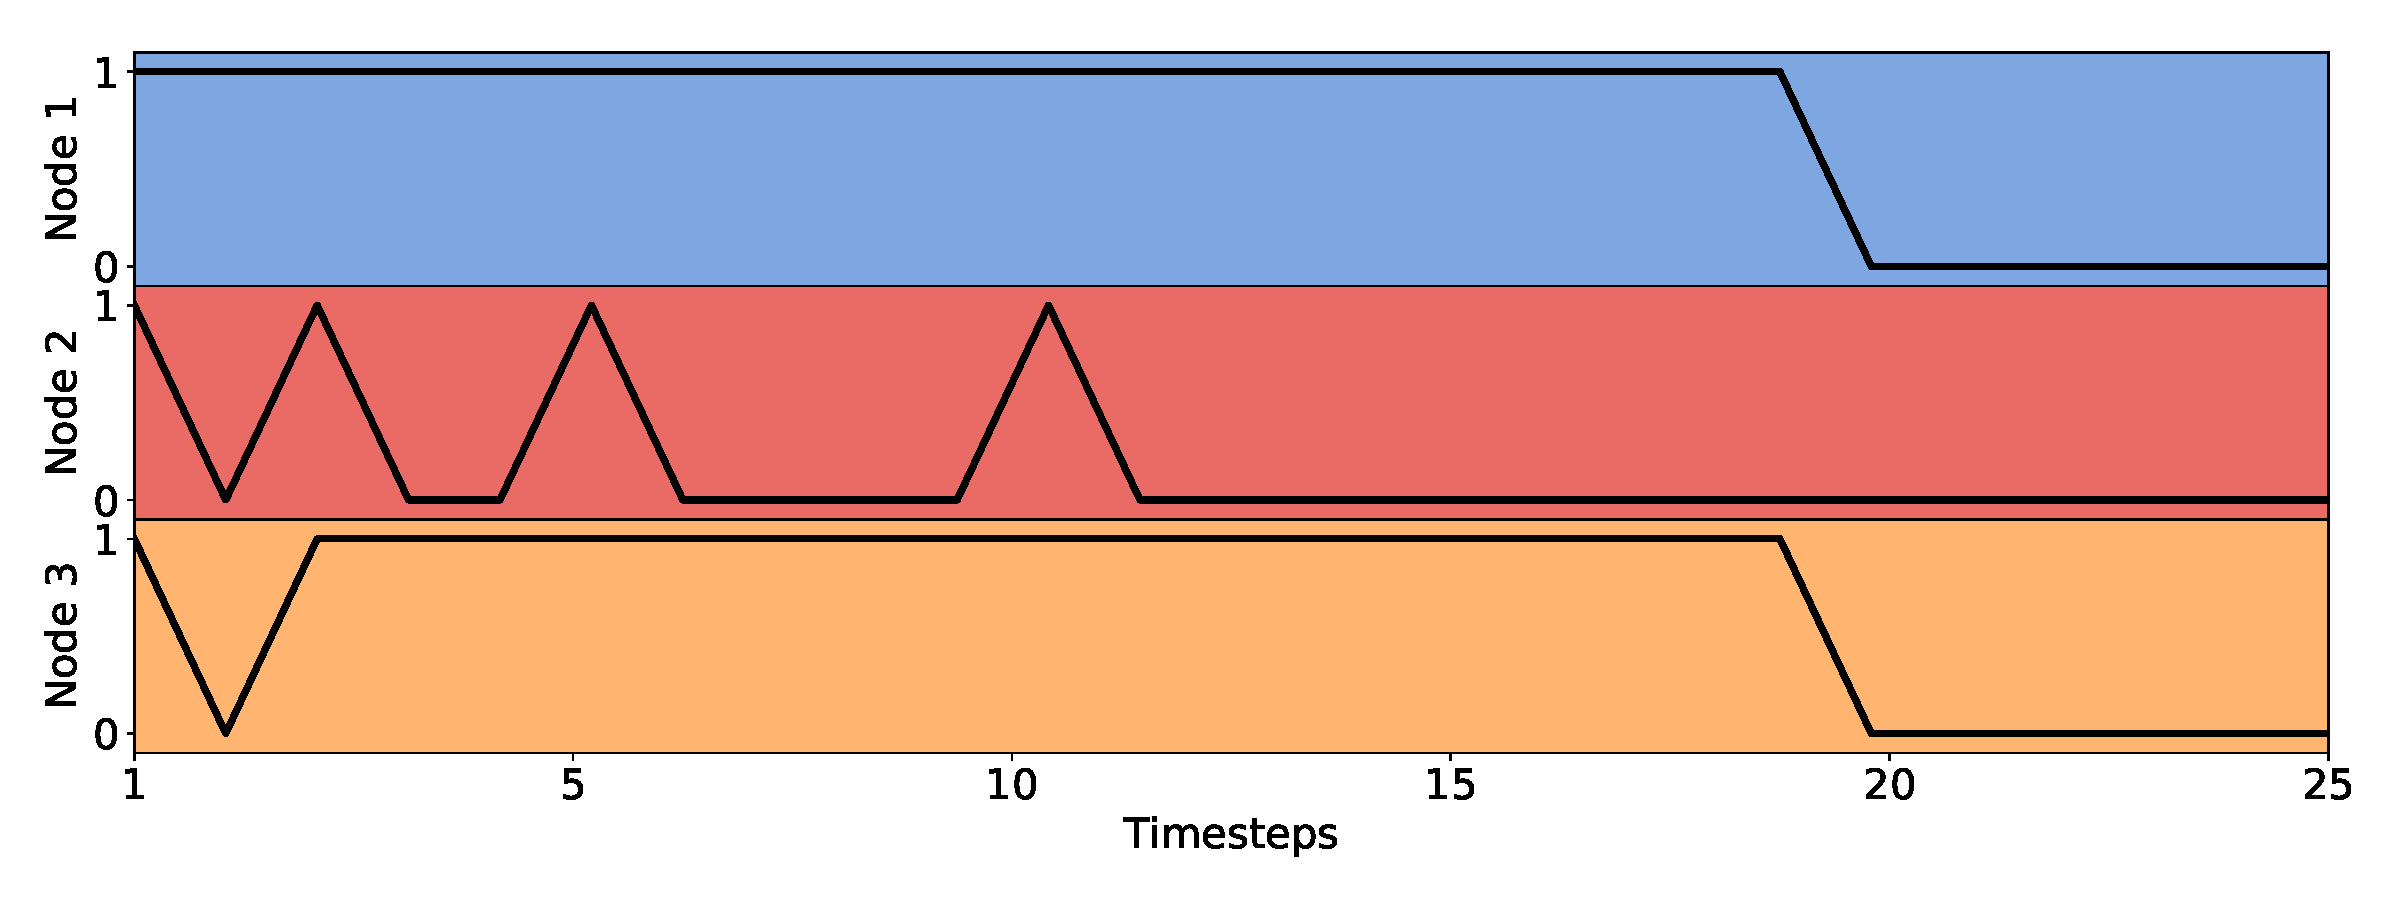
\includegraphics[width=.8\onecolwid]{img/example_skipping.pdf}
    \caption{Disentangled updates in sub-representations.}
\end{figure}

\end{alertblock}

\end{column} % End column two

% --- spacer column ---
\begin{column}{\sepwid}\end{column}

% --- begin column three ---
\begin{column}{\onecolwid}

\begin{alertblock}{\centering Evaluation Data}
Synthetic dataset:
\begin{itemize}
    \item Balanced dataset of 1000 time series, each is 100 timesteps long.
    \item Each time series is a sequence of 0's. Positive examples have a 1 at a random location. Gaussian noise is added.
    \item Remove 2 values from uniform locations from positive examples, remove 4 from negative.
    \item Impute surrogate values for missing values.
\end{itemize}
\end{alertblock}


\begin{alertblock}{\centering Results}
\begin{table}
\centering
\begin{tabular}{lc}
\toprule
Method & Accuracy\\
\midrule
Mean Imputation    & 59 $\pm$ 0.0 \\ 
Zero Imputation    & 59 $\pm$ 0.0 \\ 
Forward Imputation & 59 $\pm$ 0.0 \\ 
\midrule
SkipRNN \cite{campos2018skip}              & 59.0 $\pm$ 0.0 \\ 
GRU-D \cite{che2018recurrent}              & 80.24 $\pm$ 22.26\\ 
Mask + Mean Imp. \cite{lipton2016modeling} & 72.4 $\pm$ 26.66  \\ 
PhasedLSTM \cite{neil2016phased}           & 59 $\pm$ 0.0 \\
\midrule
Mask and diff input          & 72.40 $\pm$ 26.66 \\ 
SkipRNN + Mask               & 71.6 $\pm$ 22.83 \\ 
Mask as updates              & 59 $\pm$ 0.0 \\ 
Input mask and full-skip     & 81.5 $\pm$ 20.95 \\ 
Mask informs skipping        & 59 $\pm$ + 0.0 \\ 
Input-mask + mask-inform     & 83.6 $\pm$ 22.0 \\ 
Full-skipping w/decay impute & 91.6 $\pm$ 5.04  \\ 
MISS [proposed]              & \textbf{94.72 $\pm$ 2.69} \\
\bottomrule
\end{tabular}
\end{table}

\end{alertblock}

% --- references ---
\begin{alertblock}{References}
\tiny{\bibliographystyle{ieeetr}
\bibliography{bibliography}\vspace{1cm}}
\end{alertblock}

% --- acknowledgements ---
\begin{alertblock}{\centering Acknowledgements}
\small{\rmfamily{Thank you to the U.S. Dept. of Ed. for sponsoring this research and to the DSRG at WPI for an enriching research community.}}
\end{alertblock}

\end{column} % End of the third column

% --- spacer column ---
\begin{column}{\sepwid}\end{column}

\end{columns} % End of all the columns in the poster

\end{frame} % End of the enclosing frame
\end{document}
